\section{用户字节跨重启的完整路径}

write 返回、同次启动读回、块缓存标为 clean 和新机器进程重新读回，是四个不同
强度的结论。只有数据经过系统调用、文件对象、文件系统、缓存写回、ATA PIO 和
FLUSH，并由一个全新的 QEMU 进程重新 mount 后得到相同字节，才形成当前项目的
跨启动持久化证据。

\begin{sidewaysfigure}[p]
  \centering
  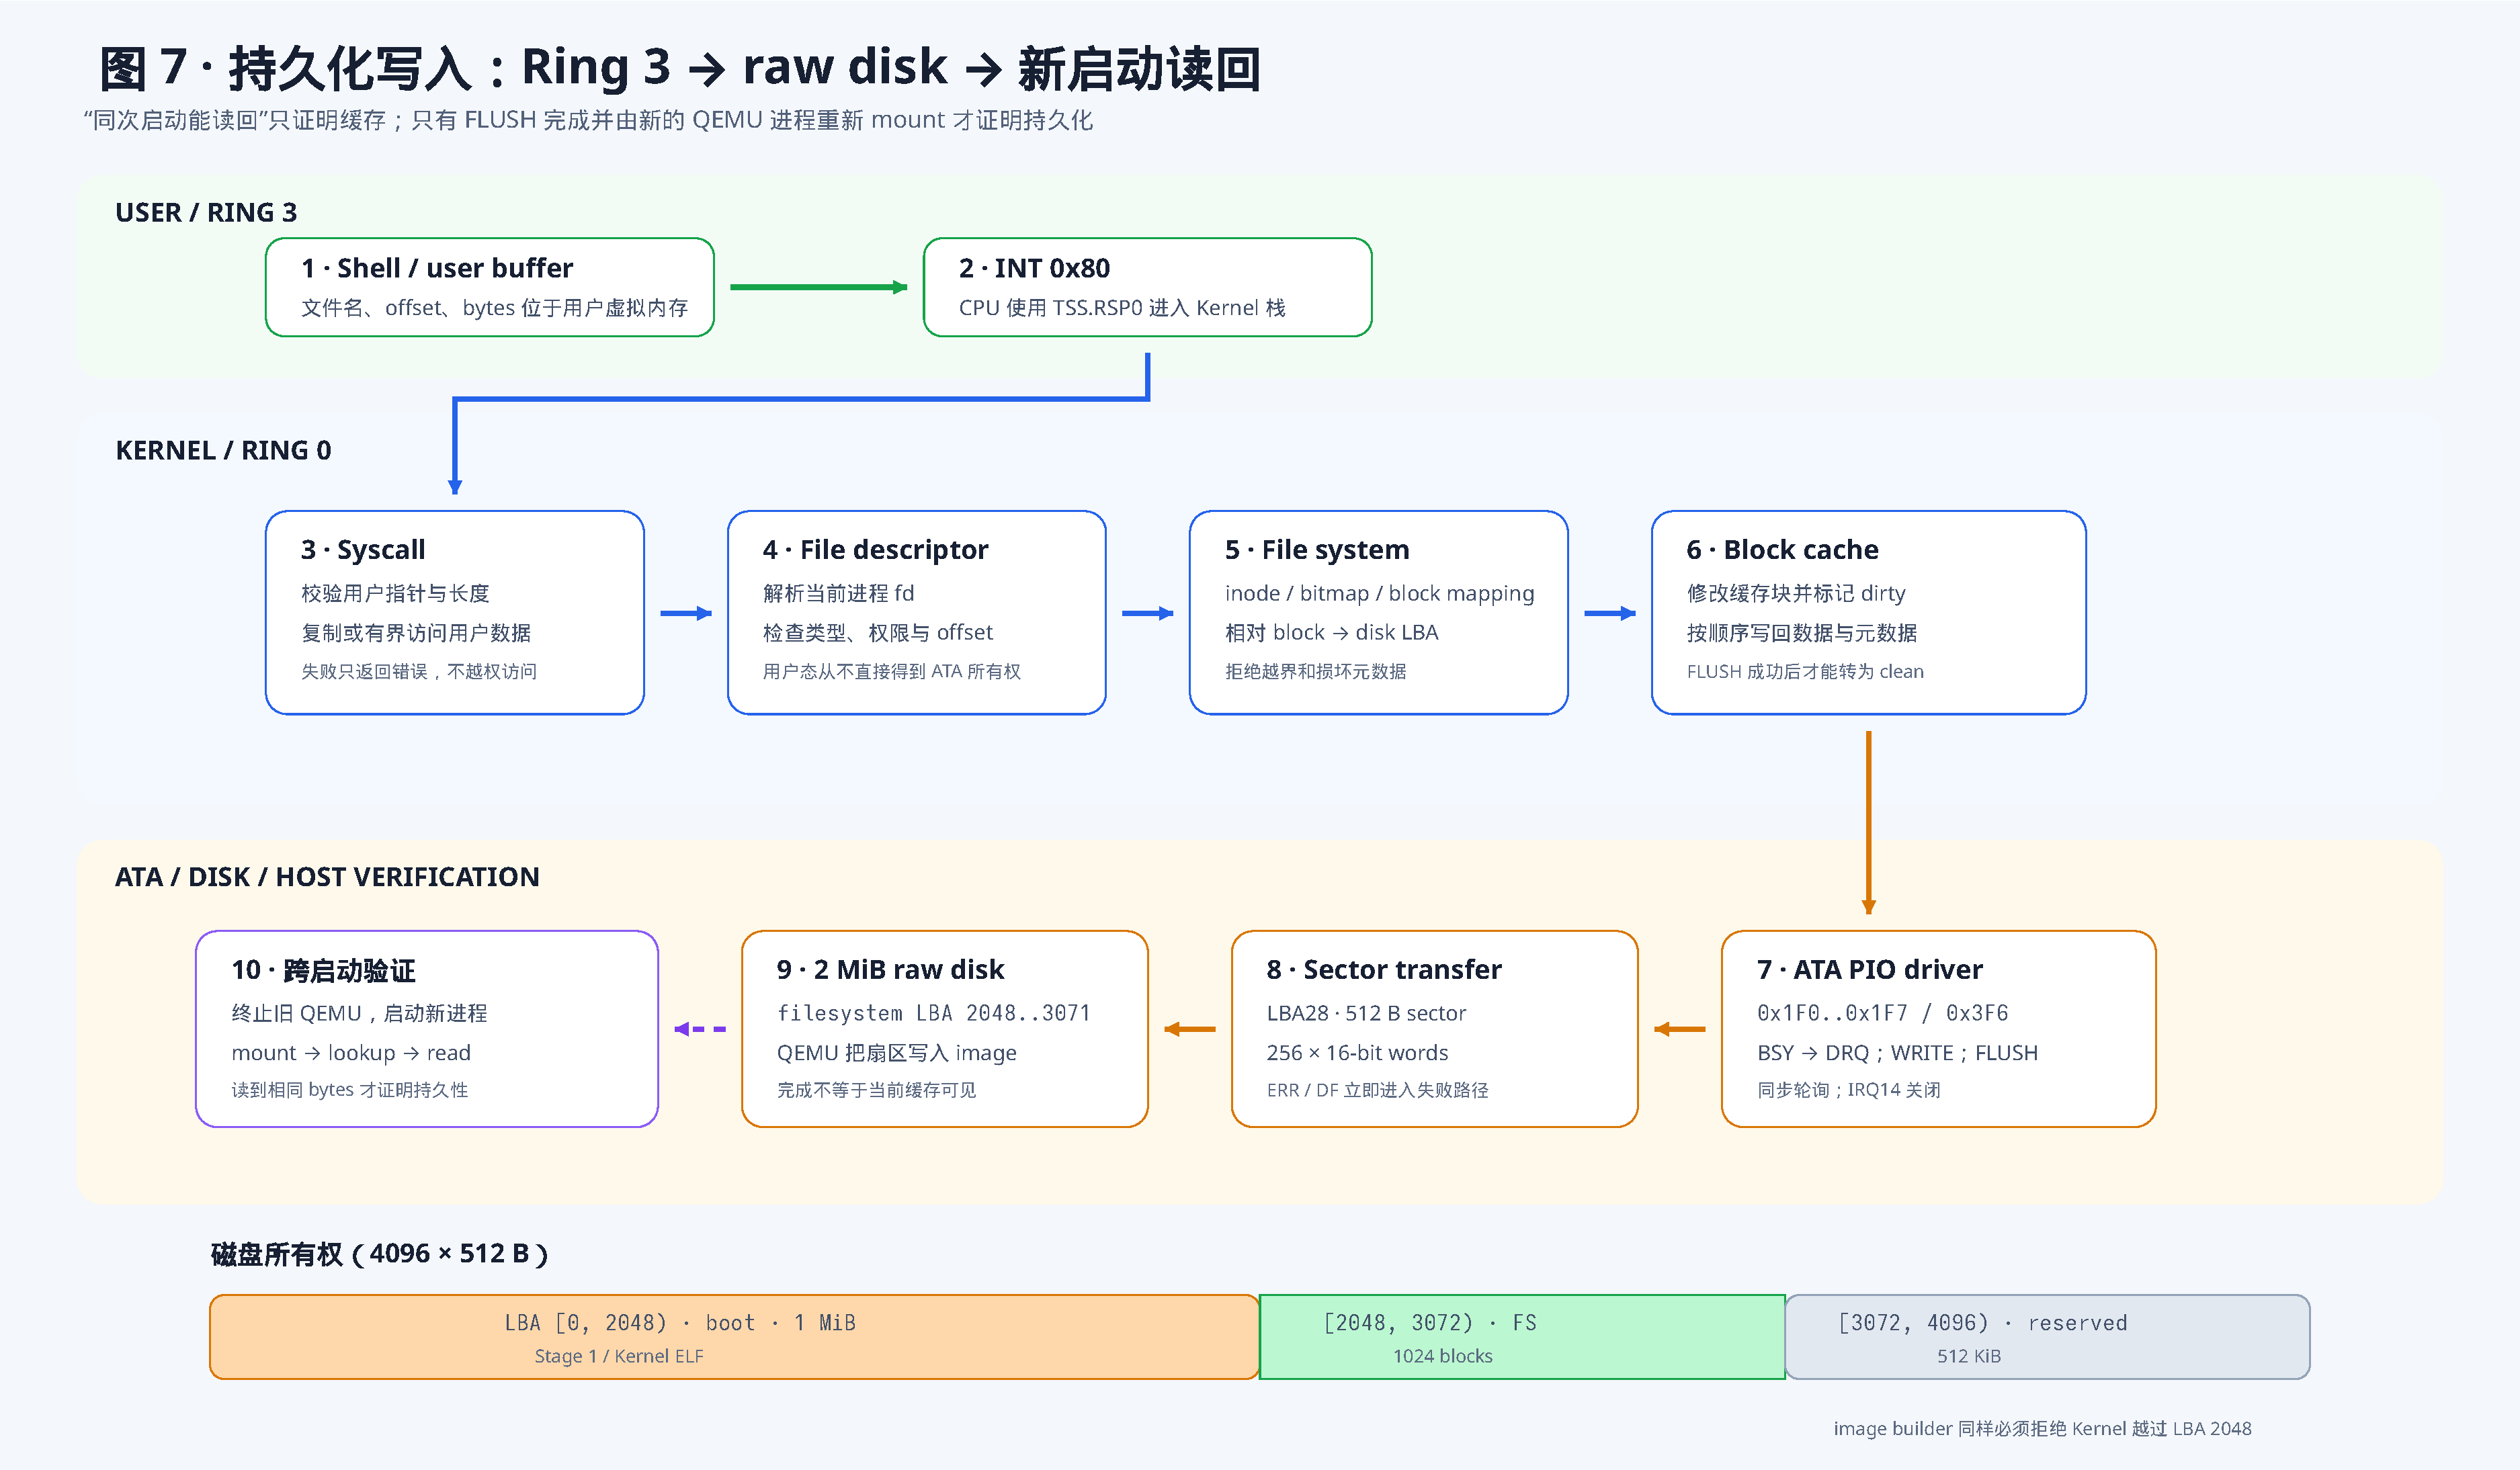
\includegraphics[width=0.96\textheight,height=0.82\textwidth,keepaspectratio]
    {figures/system_wiring/storage_persistence.pdf}
  \caption{Ring 3 文件写入到 raw disk、再由新 QEMU 启动读回的完整矢量路径。
  绿线表示用户请求，蓝线表示内核对象与数据流，橙线表示 ATA/磁盘传输，紫线
  表示跨进程验证；下方同时给出 4096 个扇区的磁盘所有权分区。}
  \label{fig:storage-persistence-full}
\end{sidewaysfigure}
\clearpage

\topic{一、先区分“可见”“已写回”和“持久”}\par
\begin{osgridlongtable}{L{0.20\linewidth}L{0.29\linewidth}L{0.31\linewidth}L{0.10\linewidth}}
结论 & 已经证明 & 还没有证明 & 强度 \\ \hline
write 返回成功 & 内核接受请求并按接口完成当前提交点 & 数据已离开全部 volatile cache & 低 \\ \hline
同次启动读回相同 & 当前内核路径能从缓存或磁盘返回字节 & 重启后仍存在 & 较低 \\ \hline
ATA WRITE 完成 & 控制器接受/处理数据传输 & 设备内部易失缓存已稳定落介质 & 中 \\ \hline
FLUSH 成功 & 设备按当前 ATA 协议完成缓存刷新 & 新启动的 mount/读取逻辑也正确 & 较高 \\ \hline
新 QEMU 进程读回 & 旧进程和所有 Guest RAM 已消失，镜像重新挂载后字节一致 & 任意断电点都有日志级原子恢复 & 当前最强 \\ \hline
\end{osgridlongtable}

\term{持久性}{persistence}表示状态在产生它的执行实例结束后仍可恢复；
\term{耐久性}{durability}通常强调已经承诺成功的数据在规定故障模型下不会
丢失。当前项目检查正常 FLUSH 后跨 QEMU 进程保存；写到任意中间位置突然
断电的恢复由后文 journal、写序和 replay 实验覆盖。

\topic{二、步骤 1--3：用户地址必须在边界上重新验证}
Shell 的文件名、offset 和 bytes 位于用户虚拟地址空间。用户程序执行
\code{INT 0x80} 后，CPU 按 IDT gate 与 TSS.RSP0 切入当前进程的 Ring 0 栈。
硬件只完成特权和栈转换，不会替 Kernel 判断指针安全。

系统调用层必须同时检查：

\begin{itemize}[leftmargin=2em]
  \item 系统调用号存在，参数个数和宽度符合 ABI；
  \item 用户地址处于允许范围，地址加长度不溢出；
  \item 每个跨页范围都具有用户访问和所需读/写权限；
  \item 字符串有最大长度和终止边界，不能无限扫描；
  \item 复制失败只返回确定错误，不把半写内核状态提交给下一层。
\end{itemize}

Kernel 不应在持有可能阻塞其他路径的锁时直接访问可故障用户页。当前模型虽比
完整 demand paging 简单，仍应维持“验证/复制用户数据”与“修改持久对象”的
清楚提交顺序。

\topic{三、步骤 4：fd 不是 inode，也不是磁盘地址}
\term{file descriptor}{文件描述符，fd}只是当前进程 FileTable 中的整数索引。
FileTable 项引用 KernelObject；文件类型进一步引用共享 FileDescription，
后者保存打开状态和当前 offset；文件系统对象再关联 inode。多层间接让复制 fd
可以共享 offset，而两次独立 open 可以得到不同 offset。

\[
\mathrm{fd}
\rightarrow \mathrm{FileTable\ entry}
\rightarrow \mathrm{KernelObject}
\rightarrow \mathrm{FileDescription}
\rightarrow \mathrm{inode/file}.
\]

每一箭头都带引用和权限语义。关闭 fd 只删除当前表项并释放相应引用；只有最后
引用离开时对象才析构。把 fd 数字直接当 inode 编号，会破坏跨进程共享、类型
检查和生命周期。

\topic{四、步骤 5：文件系统把名字和 offset 变成磁盘块}
\term{inode}{索引节点}保存文件类型、大小和数据块映射；
\term{bitmap}{位图}用 bit 记录 inode 或 block 是否已占用；
\term{directory entry}{目录项}把名称关联到 inode；
\term{superblock}{超级块}冻结磁盘格式、范围和校验。一次路径解析依次读取
目录项和 inode，文件 offset 再映射到相对 block，最后加上文件系统分区起点
得到全盘 LBA。

这些结构使用显式小端编码，不能把编译器内存中的 C++ struct 原样写盘。结构体
可能包含 padding、不同对齐或宿主字节序；磁盘格式必须对每个字段宽度、偏移、
合法范围和校验和负责。

\topic{五、步骤 6：block cache 为什么需要 dirty/clean 状态}
块缓存保留近期磁盘块的 RAM 副本，避免每次读写都发 ATA 命令。
\term{dirty}{脏}表示 RAM 副本比持久介质更新；
\term{clean}{干净}表示该副本与已确认的介质状态一致。把内存改完不应立即标
clean；只有数据、元数据按协议写出并完成必要 FLUSH，才能推进状态。

写回次序会影响故障后可解释性。若目录项先指向尚未写好的 inode，或 inode
先指向尚未分配/写好的数据块，断电后会出现悬空引用。当前固定布局使用明确的
Dirty/Clean 提交和全盘一致性检查；更完整的 v2 方案用 ordered metadata
journal 进一步定义崩溃恢复边界。

\topic{六、步骤 7--8：ATA PIO 把一个扇区变成 256 个 word}
驱动向 primary ATA 的任务文件寄存器写 LBA28、扇区数和命令，轮询 BSY、DRQ、
ERR 与 DF。数据口 \code{0x1F0} 按 16 位访问，一个 512 B 扇区需要传输
256 个 word。控制寄存器和状态寄存器仍按 8 位访问，不能为了循环方便把整组
端口都改成同一宽度。

\term{sector}{扇区}是当前 ATA 传输的 512 B 单位；
\term{LBA}{Logical Block Address}是扇区编号；
\term{filesystem block}{文件系统块}是文件系统分配和缓存单位。当前图中两者
同为 512 B，概念仍不能合并，因为未来文件系统可用多个 sector 组成一个 block，
NVMe 也有自己的 namespace 与 logical block 规格。

\topic{七、步骤 9：raw disk 是镜像容器，不等于文件系统}
\term{raw disk image}{原始磁盘镜像}按扇区保存整块虚拟磁盘，没有宿主文件系统
替 Guest 自动解释内容。v0.11 的历史 2 MiB 镜像共有
\[
4096\times512\ \mathrm{B}=2\ \mathrm{MiB}.
\]

\begin{osgridlongtable}{L{0.22\linewidth}L{0.22\linewidth}L{0.25\linewidth}L{0.21\linewidth}}
LBA 半开区间 & 大小 & 所有者 & 内容 \\ \hline
\([0,2048)\) & 1 MiB & 启动镜像布局 & Stage 1、Kernel 容器/ELF 与保留结构 \\ \hline
\([2048,3072)\) & 512 KiB & 文件系统 & 1024 个当前文件系统块 \\ \hline
\([3072,4096)\) & 512 KiB & 明确保留 & 不允许 Kernel 镜像或文件系统越界占用 \\ \hline
\end{osgridlongtable}

半开区间让长度等于 end-start，相邻区域可以无歧义拼接。镜像构建器和 Kernel
都必须拒绝越过边界；否则一次大文件写入可能覆盖下一次启动所需的 Kernel，
表面文件系统成功却让机器再也不能启动。

自 v1.6 起镜像已扩为逻辑 1 GiB 稀疏文件；v1.9 当前从 LBA 32768 起分配
固定 256 MiB rootfs。本表保留为第一版持久格式的历史基线，详细新布局见本章
后续 rootfs v2 节。

\topic{八、步骤 10：为什么必须终止旧 QEMU}
如果只在同一个 Guest 中 unmount/mount 或重新读取，RAM 中仍可能保留缓存、
对象和错误的未写回副本。自动测试先等待写入、sync 和成功标记，再终止旧 QEMU
进程；随后用同一磁盘文件启动全新的 QEMU。新 Guest 的 CPU、RAM、Kernel 堆和
块缓存均重新建立，只能从 disk image 读取状态。

新启动必须通过 superblock 验证、mount、路径查找、inode/block 读取，最终得到
精确相同字节。测试还要使用禁止标记确保没有悄悄格式化损坏磁盘、没有走错误
恢复分支，超时则视为失败而非“可能还在写”。

\topic{九、把 QEMU ATA 换成实体 NVMe 时哪些层保持}
文件描述符、FileDescription、路径、inode、bitmap、块缓存和大部分文件系统
规则可以保持；最下层块设备驱动和发现路径必须替换。DFR1142 的 M.2 M Key
连接 PCIe x1，常见 SSD 使用 NVMe，而当前 STUOS 只驱动 QEMU 的 legacy ATA
PIO。实体适配至少还需：

\begin{enumerate}[leftmargin=2.2em]
  \item 通过 UEFI/ACPI/PCIe 配置空间发现 root 与 NVMe function；
  \item 分配/读取 BAR，把控制器 MMIO 映射成正确缓存属性；
  \item 建立 admin/I/O submission 与 completion queue；
  \item 为队列和数据准备 DMA 可见物理内存，处理 doorbell 与完成中断/轮询；
  \item 把 NVMe namespace block 接到现有 BlockDevice 抽象，并重新验证
        FLUSH/持久性语义。
\end{enumerate}

所以“载板有 M.2”只证明物理插槽和 PCIe 通道存在；“Kernel 有文件系统”只证明
上层格式和对象模型存在。中间 PCIe/NVMe 驱动链没有实现时，两端不能自动接通。

\topic{十、失败现象怎样对应到十步链}\par
\begin{osgridlongtable}{L{0.25\linewidth}L{0.31\linewidth}L{0.34\linewidth}}
现象 & 最可能边界 & 应保存的证据 \\ \hline
write 立即返回参数错误 & 用户复制、fd 类型/权限或范围检查 & syscall 号、fd、长度、精确错误码 \\ \hline
同次读回正确、重启丢失 & dirty cache、ATA WRITE/FLUSH 或镜像绑定 & dirty/clean 计数、状态位、FLUSH 标记 \\ \hline
重启后自动格式化 & mount 的全零/损坏分类错误 & superblock 原始字节、CRC、禁止标记 \\ \hline
小文件正常、大文件破坏启动 & block/LBA 边界或长度溢出 & 目标半开区间、镜像审计、受影响 LBA \\ \hline
第二次 QEMU 读到旧内容 & 旧进程未终止、磁盘文件错误或 flush 未完成 & 进程边界、镜像路径/hash、完成标记 \\ \hline
随机卡在 ATA & BSY/DRQ/ERR/DF 轮询与预算 & 最后状态、命令、LBA、剩余 timeout \\ \hline
\end{osgridlongtable}

端到端测试证明整条链能协作，单元/随机测试则分别证明路径解析、位图、cache、
fd 和状态机边界。两者不能互相替代：只跑 QEMU 很难覆盖每个损坏字段，只跑
内存模型又不能证明真实 ATA 端口和跨启动镜像。
